\section{Gaussian measures on function spaces}

The priors of this chapter are Gaussian measures on infinite dimensional spaces. Let $\mu = N(0,\mathcal{C})$ be a centered Gaussian measure on a separable Hilbert space $H$ with trace class covariance $\mathcal{C}$. Its Cameron Martin space is $E = \mathcal{C}^{1/2}H$ with norm $\|h\|_E = \|\mathcal{C}^{-1/2}h\|_H$.

\begin{theorem}[Cameron Martin, Feldman and H\'ajek]
\label{thm:cameron_martin}
The shifted measure $\mu(\cdot-h)$ is equivalent to $\mu$ if $h\in E$ and mutually singular with it otherwise. For $h\in E$,
\[
\frac{\dd\mu(\cdot-h)}{\dd\mu}(x) = \exp\Big(\langle\mathcal{C}^{-1/2}h,\mathcal{C}^{-1/2}x\rangle-\frac12\|h\|_E^2\Big),
\]
where $\langle\mathcal{C}^{-1/2}h,\mathcal{C}^{-1/2}x\rangle$ is the Paley Wiener integral: the $L^2(\mu)$ limit of $\langle\mathcal{C}^{-1}h_n,x\rangle$ for any $h_n\in\mathcal{C}H$ with $h_n\to h$ in $E$. It is a centered Gaussian variable with variance $\|h\|_E^2$. Two Gaussian measures are either equivalent or mutually singular.
\end{theorem}

We quote the theorem without proof. The density is the Cameron Martin formula and the dichotomy is the Feldman H\'ajek theorem; both are proved in Bogachev~\cite{bogachev1998}.

The Cameron Martin space has $\mu$ measure zero in infinite dimensions: draws from the prior are rougher than the functions the prior considers typical shifts. The maximum a posteriori estimator is defined through the Onsager Machlup functional
\[
I(\theta) = \mathcal{V}(\theta;y)+\frac12\|\theta\|_E^2,\qquad\mathcal{V}(\theta;y) = \frac{1}{2\delta^2}\|y-\mathcal{G}(\theta)\|^2,
\]
whose minimizer over $E$ is the Tikhonov regularized solution with penalty given by the Cameron Martin norm. Dashti, Law, Stuart and Voss~\cite{dashti2013} proved that this minimizer is the limit of the centers of small balls of maximal posterior probability, which gives the maximum a posteriori estimator a measure theoretic meaning in infinite dimensions.

\section{Well posedness of the posterior}

\begin{theorem}[Stuart]
\label{thm:stuart_wellposed}
Let $\Pi$ be a probability measure on a separable Banach space $X$ and let $\mathcal{V}:X\times\R^m\to\R$ be continuous. Suppose that for every $r>0$ there are nondecreasing functions $M_1(r,\cdot)$ and $M_2(r,\cdot)$, with $M_2$ strictly positive, such that for all $\theta\in X$ and all $y,y_1,y_2\in\R^m$ of norm at most $r$,
\[
\begin{gathered}
\mathcal{V}(\theta;y)\geq-M_1(r,\|\theta\|),\\
|\mathcal{V}(\theta;y_1)-\mathcal{V}(\theta;y_2)|\leq M_2(r,\|\theta\|)\,\|y_1-y_2\|,
\end{gathered}
\]
and that, for every $r>0$, $e^{M_1(r,\|\theta\|)}\big(1+M_2(r,\|\theta\|)^2\big)$ is integrable under $\Pi$. Then $Z(y) = \int e^{-\mathcal{V}(\theta;y)}\Pi(\dd\theta)$ is positive and finite, the measure $\Pi^y$ with density $Z(y)^{-1}e^{-\mathcal{V}(\theta;y)}$ with respect to $\Pi$ is a probability measure, and for every $r>0$ there is $C$ such that
\[
d_{\mathrm{Hell}}\big(\Pi^y,\Pi^{y'}\big)\leq C\|y-y'\|
\]
for all $y,y'$ of norm at most $r$.
\end{theorem}

This is a special case of the well posedness theorems of Dashti and Stuart~\cite{dashti2017}. The theorem holds for data in a Banach space. For a Gaussian prior the integrability condition is checked with Fernique's theorem, which gives $\int e^{\varepsilon\|\theta\|^2}\Pi(\dd\theta)<\infty$ for small $\varepsilon>0$. The condition holds for the potential $\mathcal{V}(\theta;y) = \frac{1}{2\delta^2}\|y-\mathcal{G}(\theta)\|^2$ when $\mathcal{G}$ is continuous and grows at most polynomially in $\|\theta\|$, with $M_1 = 0$ and $M_2(r,s) = \delta^{-2}\big(r+\sup_{\|\theta\|\leq s}\|\mathcal{G}(\theta)\|\big)$.

\begin{proof}[Sketch]
Fix $r>0$ and write $M_i$ for $M_i(r,\|\theta\|)$. The lower bound gives $Z(y)\leq\int e^{M_1}\dd\Pi<\infty$. Take a point $\theta_0$ in the support of $\Pi$. By continuity and the Lipschitz bound in $y$, $\mathcal{V}$ is bounded above, uniformly for $\|y\|\leq r$, on a neighborhood of $\theta_0$, and the neighborhood has positive prior mass, so $Z(y)$ is bounded away from zero. For $a,b\geq-M$ one has $|e^{-a}-e^{-b}|\leq e^M|a-b|$ and $|e^{-a/2}-e^{-b/2}|\leq\frac12e^{M/2}|a-b|$. Hence
\[
\begin{gathered}
|Z(y)-Z(y')|\leq\|y-y'\|\int e^{M_1}M_2\,\dd\Pi,\\
\int\big(e^{-\mathcal{V}(\theta;y)/2}-e^{-\mathcal{V}(\theta;y')/2}\big)^2\,\dd\Pi\leq\frac14\|y-y'\|^2\int e^{M_1}M_2^2\,\dd\Pi,
\end{gathered}
\]
and both integrals are finite by assumption. The squared Hellinger distance is at most a constant times the sum of the second integral and $|Z(y)-Z(y')|^2$, with a constant that depends on the lower bound for $Z$, and the claim follows.
\end{proof}

The map from data to the least squares initial condition is discontinuous, since the backward heat equation is ill posed in Hadamard's sense, but the map from data to posterior is Lipschitz in the Hellinger metric. Bayesian inversion is well posed where deterministic inversion is not, because it returns a measure that spreads its mass over the directions the data cannot determine.

\section{Dimension robust sampling}\label{sec:dimrobust}

Standard random walk Metropolis algorithms degenerate as the discretization of a function space problem is refined: the acceptance rate falls to zero unless the step size shrinks with the dimension. The preconditioned Crank Nicolson proposal of Cotter, Roberts, Stuart and White~\cite{cotter2013} avoids this. With prior $N(0,\mathcal{C})$, propose
\[
\theta' = \sqrt{1-\beta^2}\,\theta+\beta\,\xi,\qquad\xi\sim N(0,\mathcal{C}),
\]
and accept with probability $\min\{1,\exp(\mathcal{V}(\theta;y)-\mathcal{V}(\theta';y))\}$. The proposal is reversible with respect to the prior, so the acceptance probability involves only the likelihood, and the algorithm is well defined on the infinite dimensional space. Hairer, Stuart and Vollmer~\cite{hairer2014} proved that for a large class of target measures its Wasserstein spectral gap is bounded below independently of the discretization, and that this gap implies a spectral gap in $L^2$. The algorithm is an instance of the general principle of this book: a Markov chain that preserves the reference measure exactly, here the Gaussian prior, and corrects only for the tilt, mirrors the structure of Gibbs conditioning, in which the reference measure is fixed and only the constraint changes.

\section{A simulated example in two dimensions}\label{sec:simns2d}

Figure~\ref{fig:ns2d} shows a pseudospectral solution of the two dimensional vorticity equation, started from ten Gaussian vortices of random sign and strength. Isolated vortices persist, vortices of opposite sign close to one another are sheared into filaments, and viscosity thins the filaments. Kraichnan, Leith and Batchelor~\cite{kraichnan1967,leith1968,batchelor1969} predicted that in two dimensions energy moves to large scales and enstrophy to small scales, a dual cascade. The lower panels of the figure show the energy and enstrophy spectra, summed over shells of the wavenumber (the caption gives the definition). They show the two directions of the dual cascade only in part within $t=5$. The energy at $k=1$ rises from $0.0265$ to $0.0315$, which viscosity alone cannot do, while the total energy falls by $11$ percent, and the share of the energy at $k\le3$ rises from $0.82$ to $0.87$, so energy moves to large scales. The share of the enstrophy at $k\ge16$ grows from $5\times10^{-7}$ to $2.4\times10^{-3}$, so some enstrophy moves to small scales, but the total enstrophy falls by $32$ percent and its mean wavenumber does not rise, from $3.9$ to $3.8$. Three times of one flow do not show an inertial range.

\begin{figure}[t]
\centering
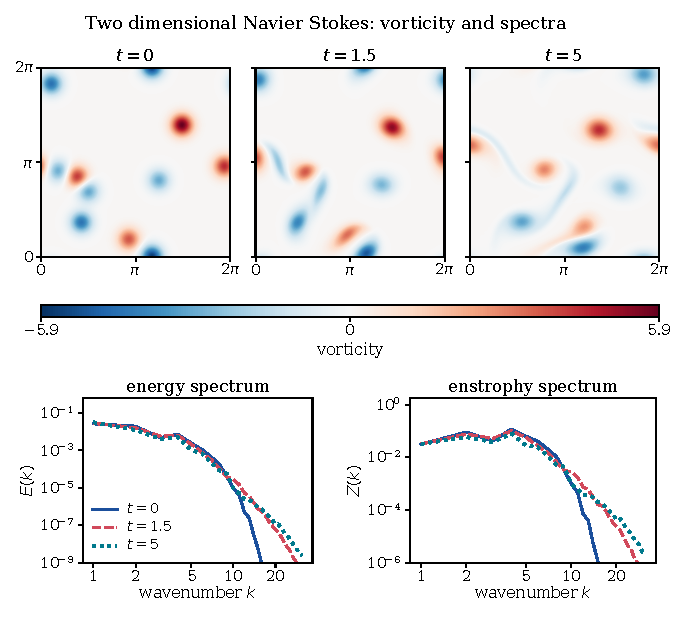
\includegraphics{ns2d}
\caption{Top: vorticity of a two dimensional Navier Stokes flow on the torus $[0,2\pi]^2$ with viscosity $\nu = 2\times10^{-3}$ at times $t = 0$, $1.5$ and $5$, started from ten Gaussian vortices of random sign. Red is positive and blue is negative vorticity (both print dark in grayscale), on one symmetric color scale for the three panels, with limits $\pm5.87$, the largest absolute value of the initial vorticity. Bottom: the energy spectrum $E(k)$ and the enstrophy spectrum $Z(k)$ per unit area at the same times, on logarithmic axes; with $\hat\omega_j$ the Fourier coefficients of the vorticity, $E(k)$ is the sum of $\frac12|\hat\omega_j|^2/|j|^2$ and $Z(k)$ the sum of $\frac12|\hat\omega_j|^2$ over the wavenumbers $j$ with $|j|$ rounded to $k$. The solution is computed by a dealiased pseudospectral method with fourth order Runge Kutta time stepping on a $96\times96$ grid.}
\label{fig:ns2d}
\end{figure}

We computed the inverse problem for a smaller flow than the one of Figure~\ref{fig:ns2d}, with a coarser grid and a larger viscosity, so that the posterior could be sampled exactly. The unknown is the initial vorticity $\omega_0=\sum_{0<|k|_\infty\le6}c_ke^{ik\cdot x}$ on $\T^2$, with $c_{-k}=\bar c_k$, which has $168$ real coefficients. The prior makes the coefficients independent and Gaussian with $\E|c_k|^2=(1+|k|^2)^{-2}$, a Mat\'ern type prior of smoothness index $1$ whose pointwise standard deviation is $1.47$. The data are the values of $\omega(T)$ at time $T=3$ at $16\times16$ equally spaced sensors, with independent Gaussian noise of standard deviation $\delta=0.25$, for viscosity $\nu=0.01$. The forward map is a dealiased pseudospectral solver with fourth order Runge Kutta steps of size $0.025$ on a $32\times32$ grid. The truth is five Gaussian vortices $a\,e^{-r^2/0.5}$, with amplitudes $a$ of both signs between $2.5$ and $6$ in absolute value, projected on the $168$ modes (Figure~\ref{fig:ns2d_posterior_data}), so that the model is correctly specified. The data were generated on a $64\times64$ grid with half the time step, not on the grid of the posterior, so that there is no inverse crime: the two solutions differ at the sensors by $0.03$ in root mean square, one ninth of $\delta$.

\begin{figure}[t]
\centering
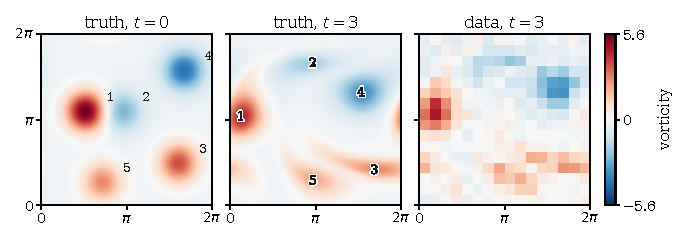
\includegraphics{ns2d_posterior_data}
\caption{Truth and data of the simulated inverse problem. Left: the initial vorticity of the truth, five Gaussian vortices numbered $1$ to $5$. Middle: the truth at the observation time $t=3$; the numbers mark where the five vortices have gone. Right: the data. One color scale for the three panels.}
\label{fig:ns2d_posterior_data}
\end{figure}

We found the maximum of the posterior density by a Levenberg Marquardt iteration, formed the Gauss Newton Hessian there, and sampled the posterior exactly by Hamiltonian Monte Carlo~\cite{duane1987,neal2011} in coordinates in which that Hessian is the identity. The gradient of the log posterior is the reverse mode derivative of the solver. Four chains were started from independent draws of the prior, and each ran $400$ warmup iterations, with the step size set by dual averaging~\cite{hoffman2014}, followed by $1000$ iterations with a random number of leapfrog steps. The mean acceptance probability was $0.77$. The largest rank normalized split $\widehat R$~\cite{vehtari2021} over the $168$ coefficients is $1.010$, and the smallest bulk effective sample size is $552$ out of $4000$ draws. The four chains reach the same posterior, and three further optimizations started from other prior draws end at the same maximum, so that we found no sign of several modes. That says nothing about regimes with a lower viscosity, a longer observation time or fewer sensors, which we did not compute. On the linear problem obtained by dropping the nonlinear term, whose posterior is Gaussian and known in closed form, the same sampler, with four chains of $300$ warmup and $600$ retained iterations, has $\widehat R\le1.009$ and reproduces the standard deviations of all $168$ coefficients to within $6$ percent, the largest of $168$ Monte Carlo errors of about $2$ percent each.

\begin{figure}[t]
\centering
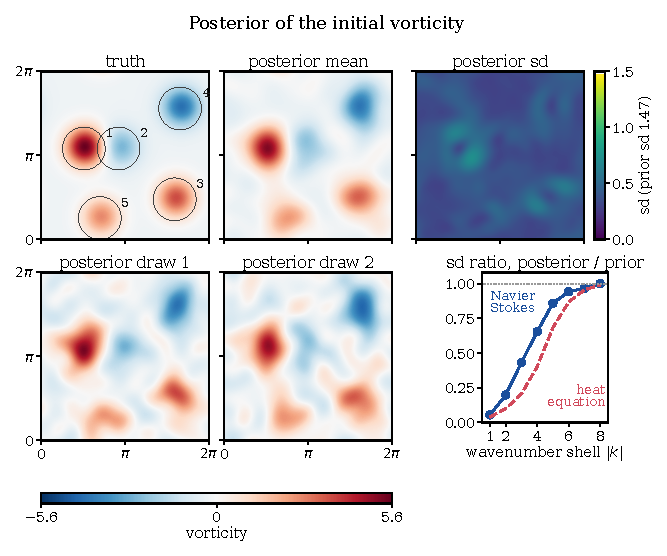
\includegraphics{ns2d_posterior}
\caption{Posterior of the initial vorticity for the data of Figure~\ref{fig:ns2d_posterior_data}, from four Hamiltonian Monte Carlo chains. Top: the truth, with the five discs of radius $0.8$ on which circulations are computed, the posterior mean, and the pointwise posterior standard deviation on a color scale from zero to the prior standard deviation $1.47$. Bottom: two posterior draws on the color scale of the truth, and the ratio of posterior to prior standard deviation of the Fourier coefficients by wavenumber shell (the square root of the ratio of the summed variances over the modes with $|k|$ rounded to $m$), for the nonlinear problem and for the problem with the nonlinear term dropped.}
\label{fig:ns2d_posterior}
\end{figure}

Figure~\ref{fig:ns2d_posterior} shows the posterior. The posterior mean recovers the five vortices, the draws differ from it in a fine scale texture that the data do not constrain, and the standard deviation of the field is at most $0.74$, against $1.47$ for the prior. By wavenumber shell, the ratio of the posterior to the prior standard deviation of the coefficients, pooled over the shell as in the caption, is $0.05$, $0.20$ and $0.43$ for $|k|=1,2,3$, $0.65$ at $|k|=4$ and $0.86$ at $|k|=5$, and at least $0.94$ for $|k|\ge6$: the large scales are learned and the small scales are left at the prior. With the nonlinear term dropped, the vorticity equation becomes the heat equation, and the same prior, sensors and noise give a diagonal posterior that learns more at every wavenumber, with ratios $0.04$, $0.10$, $0.20$, $0.40$ and $0.68$ for $|k|=1,\dots,5$. The nonlinear posterior is not diagonal: $158$ of the $14028$ pairs of coefficients have a posterior correlation above $0.3$ in absolute value, and the largest is $0.67$.

\begin{table}[t]\centering\footnotesize\setlength{\tabcolsep}{5pt}
\caption{Posterior mean and standard deviation (sd) of the energy and of the circulations of the initial vorticity. The prior standard deviation is $14.3$ for the energy, estimated from $20000$ prior draws, and $2.36$ for every circulation. The circulation is the integral of $\omega_0$ over the disc of radius $0.8$ around vortex $j$. The position error is the root mean square distance, over posterior draws, between the location of the extremum of $\omega_0$ in that disc and its location in the truth; under the prior it is between $0.72$ and $0.73$ for every vortex. The elongation is the ratio of the principal axes of the region in which vortex $j$, advected to $t=3$ separately by the velocity of the whole field, exceeds a fifth of its maximum; it is $1$ at $t=0$.}\label{tab:ns2d_posterior}
\begin{tabular}{@{}lrrrrr@{}}
\toprule
Functional & Truth & Mean & Sd & Position error & Elongation\\
\midrule
Energy & $12.62$ & $13.03$ & $0.42$ & & \\
Circulation 1 & $5.88$ & $5.78$ & $0.19$ & $0.14$ & $1.33$\\
Circulation 2 & $-2.37$ & $-2.39$ & $0.24$ & $0.32$ & $2.43$\\
Circulation 3 & $4.02$ & $3.85$ & $0.19$ & $0.20$ & $4.52$\\
Circulation 4 & $-5.06$ & $-5.03$ & $0.16$ & $0.26$ & $1.31$\\
Circulation 5 & $2.88$ & $2.70$ & $0.16$ & $0.26$ & $2.17$\\
\bottomrule
\end{tabular}
\end{table}

Table~\ref{tab:ns2d_posterior} gives the posterior of the energy $\frac12\int_{\T^2}|u_0|^2\dd x$ of the initial velocity and of the circulations on the discs of Figure~\ref{fig:ns2d_posterior}. The standard deviation of the energy is $3$ percent of its prior value and those of the circulations are $7$ to $10$ percent of theirs. The truth is within $1.2$ posterior standard deviations of the posterior mean for each of the six, and the posterior of the energy is close to normal, with skewness $0.10$ and excess kurtosis $-0.03$. We repeated the computation with the same noise draw rescaled to $\delta=0.5$ and $\delta=0.125$, with $300$ warmup and $600$ retained iterations per chain, $\widehat R\le1.03$ and a bulk effective sample size of at least $196$ for the coordinates; the Monte Carlo error of each standard deviation of a functional below is $2$ to $4$ percent. The standard deviation of the energy is $0.83$, $0.42$ and $0.21$ for $\delta=0.5$, $0.25$ and $0.125$, proportional to $\delta$ within $2$ percent, and those of the circulations of vortices 1, 3, 4 and 5 scale as $\delta^s$ over the same range with $s$ between $0.90$ and $1.07$. The circulation of vortex 2, the weakest, scales as $\delta^{0.73}$, and the point value of $\omega_0$ at the center of vortex 1, which depends on small scales, as $\delta^{0.68}$. A standard deviation proportional to $\delta$, together with a nearly normal posterior, is what a Bernstein von Mises theorem leads one to expect of a smooth functional. In this experiment the energy has both. One experiment says nothing about rates. The Gaussian approximation at the maximum of the posterior gives standard deviations of these six functionals that are $4$ to $11$ percent too small, and the importance weights of its draws have an effective sample size of $0.9$ percent, so that as a measure on $\R^{168}$ it is not close to the posterior.

The five vortices are not determined equally well. Advected separately by the velocity of the whole field, vortices 3 and 5 are drawn by $t=3$ into thin arcs and vortex 2 into a flat band, while vortices 1 and 4 stay compact (Table~\ref{tab:ns2d_posterior}). The standard deviation of the circulation of vortex 2 is the largest of the five, and so is the error of its position. But vortex 3, the most elongated, has the circulation standard deviation of the compact vortex 1, and vortex 5, which is also drawn into an arc, has a circulation standard deviation as small as that of the compact vortex 4. Vortex 2 is also the weakest of the five, so that this experiment shows no clear effect of filamentation on how well a vortex is determined.


\section*{Exercises}
\begin{enumerate}
\item In the heat equation sequence model, derive the posterior mean and variance of $\theta_k$.
\item Show that the functional $L\theta = \theta_1$ satisfies the summability condition of Theorem~\ref{thm:heat_rates} and compute its asymptotic variance.
\item Prove that the preconditioned Crank Nicolson proposal is reversible with respect to $N(0,\mathcal{C})$.
\item Show that a traveling front $U(x-ct)$ of the Fisher Kolmogorov equation satisfies $DU''+cU'+rU(1-U) = 0$, and that rescaling the variable by $\sqrt{D/r}$ leaves the single parameter $c/\sqrt{rD}$.
\item Compute the Cameron Martin norm of a smooth function $h$ with $h(0) = 0$ under the Brownian motion prior on $[0,1]$.
\end{enumerate}
